\chapter{Examples}

In this chapter we show how to use Sundance to solve several linear and
nonlinear PDEs. Features are discussed as they arise in the problems.
For a more systematic survey of features and syntax, see the User's Guide.
In each of the examples that follow, we show how to set up a problem
by defining the mesh,
the locations where BCs are to be applied, all variables and operators,
and the equation set and BCs. We then show configuration of a solver
(linear or nonlinear depending on the problem), solution of the problem,
and output. 

Source code as well as associated files for meshes and solver parameters
for all of these examples can be found can be found in the subdirectory
\begin{verbatim}
examples-tutorial
\end{verbatim}
of the Sundance distribution.


\section{Example: Potential Flow Past an Elliptical Post}
\label{PotentialFlowExample}
We'll begin with what is perhaps the simplest PDE to solve numerically: 
Laplace's equation $\nabla^2 u = 0$. Though simple, we can illustrate much of
Sundance syntax with the problem. The Laplace equation is ubiquitous in
applications (see, e.g, \cite{FeynmanII}), one of which is incompressible, 
irrotational flow. Incompressibility and
irrotationality require that the velocity field $\uvec$ satisfy 
\begin{eqnarray}
\nabla\cdot\uvec&=0\\
\nabla\times\uvec&=0,
\end{eqnarray}
from which it follows that the velocity is the gradient of a scalar
potential
\begin{equation}
\uvec=\nabla\phi
\end{equation}
and
\begin{equation}
-\nabla^2\phi = 0.
\end{equation}
We have used a negative sign above in order to get 
a positive definite operator.

\begin{figure}[p]
\epsfig{file=postGeom.ps, width=6.0in}
\caption{Domain for potential flow example. The numbers correspond to the side
set labels.}
\label{PostGeom}
\end{figure}

We will consider flow past the post shown in figure~\ref{PostGeom}. We imagine
the post placed in a wind tunnel with impenetrable walls and a constant
inlet potential $\phi_0$ which we can choose to be zero. 
We also need a downstream boundary condition. The
correct downstream boundary condition is constant velocity at infinity;
a reasonable approximation usable in a finite domain
is to assume the potential increases
linearly towards some constant potential $\phi_{out}$ some distance $L$
downstream from the outlet.\footnote{It is reasonable to use such a BC for
the inlet as well; however, we use the Dirichlet BC $\phi=0$ here in order
to show how to set up Dirichlet BCs in Sundance.} 
We therefore have BCs
\begin{eqnarray}
\phi&=0 \;\; \text{at inlet,}\\
{\bf\hat n}\cdot\nabla\phi&=0 \;\; \text{at walls,}\\
{\bf\hat n}\cdot\nabla\phi&=\frac{\phi_1-\phi}{L} \;\; \text{at outlet.}\\
\end{eqnarray}

With the equation and BCs in hand, we can write the potential flow problem
in weak form. Multiplying by a test function ${\hat\phi}$ and integrating
by parts, we have
\begin{equation}
\int_\text{interior} \nabla{\hat\phi}\cdot\nabla\phi 
-\int_\text{boundary} {\hat\phi} \nabla\phi \cdot {\bf\hat n} = 0. 
\end{equation}
We now use the BCs to rewrite the boundary term. On the tunnel walls, 
${\bf\hat n}\cdot\nabla\phi=0$, so the boundary term vanishes. Applying the
BC at the outlet and ignoring for the moment the inlet BC, we have
\begin{equation}
\int_\text{interior} \nabla{\hat\phi}\cdot\nabla\phi 
-\int_\text{outlet} \frac{1}{L}{\hat\phi}\left(\phi_{out} - \phi\right) 
-\int_\text{inlet} {\hat\phi} \nabla\phi \cdot {\bf\hat n} = 0. 
\end{equation}
At the inlet, we impose the Dirichlet BC $\phi=0$ instead of the PDE.
The Dirichlet BC can be written weakly as
\begin{equation}
\int_\text{inlet} {\hat\phi} \phi = 0
\end{equation}
for all test functions ${\hat\phi}$ that are nonzero on the inlet.
We therefore have two cases
\begin{equation}
\begin{cases}
\int_\text{interior} \nabla{\hat\phi}\cdot\nabla\phi 
-\int_\text{outlet} \frac{1}{L}{\hat\phi}\left(\phi_{out} - \phi\right) = 0
& \forall {\hat \phi}\;\text{such that}\;
 {\hat \phi} = 0 \;\; \text{on inlet}\\
\\
\int_\text{inlet} {\hat\phi} \phi = 0
& \forall {\hat \phi}\; \text{such that}\;
{\hat \phi} \ne 0 \;\; \text{on inlet}\\
\end{cases}
\end{equation}
It will be shown below how these two cases are distinguished in Sundance.